\documentclass[11pt,letterpaper]{report}

% ---------- Codificación e Idioma ----------
\usepackage[utf8]{inputenc}
\usepackage[T1]{fontenc}
\usepackage[spanish,es-nodecimaldot,es-noshorthands]{babel}
\usepackage{lmodern}
\usepackage[margin=2.2cm,headheight=14pt]{geometry}

% ---------- Gráficos, Tablas y Formato ----------
\usepackage{graphicx}
\usepackage{float}
\usepackage{array}
\usepackage{booktabs}
\usepackage{longtable}
\usepackage{tabularx}
\usepackage{makecell}
\usepackage{seqsplit}
\newcolumntype{L}[1]{>{\raggedright\arraybackslash}p{#1}}
\usepackage[table]{xcolor}
\usepackage{amsmath,amssymb}
\usepackage{enumitem}
\usepackage{fancyhdr}
\usepackage{titlesec}
\usepackage{listings}
\usepackage{hyperref}

% ---------- TikZ para UML 2.5 y CFGs McCabe ----------
\usepackage{tikz}
\usetikzlibrary{arrows.meta,positioning,calc,shapes.geometric,shapes.multipart,fit,backgrounds}

% ---------- Paleta Corporativa y Académica ----------
\definecolor{usaVerde}{HTML}{1B5E20}
\definecolor{usaVerdeClaro}{HTML}{E8F5E9}
\definecolor{usaAzul}{HTML}{0D47A1}
\definecolor{usaAzulClaro}{HTML}{E3F2FD}
\definecolor{usaGris}{HTML}{37474F}
\definecolor{usaFondoCodigo}{HTML}{F8FAFC}
\definecolor{usaBordeCodigo}{HTML}{CBD5E1}
\definecolor{usaRojo}{HTML}{B71C1C}
\definecolor{usaAmbar}{HTML}{E65100}

\hypersetup{
    colorlinks=true,
    linkcolor=usaAzul,
    urlcolor=usaAzul,
    citecolor=usaVerde,
    pdftitle={Informe Final Sesion 6 - AgriTech Precision (Grupo 2)},
    pdfauthor={Grupo 2 - Universidad Sergio Arboleda}
}

\pagestyle{fancy}
\fancyhf{}
\fancyhead[L]{\small\color{usaGris}AgriTech Precision --- Grupo 2 (PCIA5008)}
\fancyhead[R]{\small\color{usaGris}Entrega Final (Sesión 6)}
\fancyfoot[C]{\thepage}
\renewcommand{\headrulewidth}{0.4pt}

\titleformat{\chapter}[display]
  {\normalfont\huge\bfseries\color{usaVerde}}
  {\chaptername\ \thechapter}{10pt}{\Huge}
\titlespacing*{\chapter}{0pt}{-10pt}{18pt}

\titleformat{\section}
  {\normalfont\Large\bfseries\color{usaAzul}}
  {\thesection}{1em}{}
\titleformat{\subsection}
  {\normalfont\large\bfseries\color{usaGris}}
  {\thesubsection}{1em}{}

\newcolumntype{Y}{>{\raggedright\arraybackslash}X}
\renewcommand{\tablename}{Tabla}
\renewcommand{\figurename}{Figura}

% ---------- Configuración de Listings ----------
\lstset{
    backgroundcolor=\color{usaFondoCodigo},
    basicstyle=\ttfamily\footnotesize,
    columns=fullflexible,
    keepspaces=true,
    breaklines=true,
    frame=single,
    rulecolor=\color{usaBordeCodigo},
    keywordstyle=\color{usaAzul}\bfseries,
    commentstyle=\color{usaVerde}\itshape,
    stringstyle=\color{usaAmbar},
    numbers=left,
    numberstyle=\tiny\color{usaGris},
    numbersep=6pt,
    showstringspaces=false,
    tabsize=4,
    literate=
      {á}{{\'a}}1 {é}{{\'e}}1 {í}{{\'i}}1 {ó}{{\'o}}1 {ú}{{\'u}}1
      {Á}{{\'A}}1 {É}{{\'E}}1 {Í}{{\'I}}1 {Ó}{{\'O}}1 {Ú}{{\'U}}1
      {ñ}{{\~n}}1 {Ñ}{{\~N}}1 {°}{{\textdegree}}1
      {≤}{{$\le$}}1 {≥}{{$\ge$}}1 {→}{{$\rightarrow$}}1
}

\begin{document}

% ==============================================================================
% PORTADA OFICIAL
% ==============================================================================
\begin{titlepage}
    \centering
    
\includegraphics[width=0.28\textwidth]{./figures/sergio_arboleda.png}\\[0.5cm]
    {\Large \textbf{UNIVERSIDAD SERGIO ARBOLEDA}}\\[0.15cm]
    {\large ESCUELA DE CIENCIAS EXACTAS E INGENIERÍA}\\
    {\normalsize PROGRAMA DE CIENCIAS DE LA COMPUTACIÓN E INTELIGENCIA ARTIFICIAL}\\[1.2cm]

    {\color{usaVerde}\rule{\textwidth}{1.5pt}}\\[0.4cm]
    {\Huge \textbf{ENTREGA FINAL (SESIÓN 6): AGRITECH PRECISION}}\\[0.3cm]
    {\Large Monitoreo Agrícola IoT, Riego Automatizado y Aseguramiento de Calidad (SQA)}\\[0.3cm]
    {\color{usaVerde}\rule{\textwidth}{1.5pt}}\\[1.0cm]

    \textbf{Proyecto \#2 --- Grupo 2}\\[0.5cm]
    {\large
    \textbf{Juan David López Yara} (Scrum Master)\\
    \textbf{Santiago José Rodríguez Gutiérrez} (Developer)\\
    \textbf{Camilo Andrés Díaz García} (Developer)\\
    \textbf{Roger Adrián Bohórquez Moreno} (Product Owner)
    }\\[1.4cm]

    \textbf{Docente:}\\
    {\large Juan David Rodríguez Martínez}\\[0.4cm]
    \textbf{Asignatura:}\\
    {\large Ingeniería de Software I (PCIA5008)}\\[1.4cm]

    \vfill
    {\large Bogotá D.C., Colombia\\
    Noviembre de 2026}
\end{titlepage}

\tableofcontents
\clearpage

% ==============================================================================
% CAPÍTULO 1: INGENIERÍA DE REQUISITOS (ISO/IEC/IEEE 29148) Y GLOSARIO
% ==============================================================================
\chapter[Ingeniería de Requisitos (ISO/IEC/IEEE 29148) y Modelo de Dominio]{Ingeniería de Requisitos\\ (ISO/IEC/IEEE 29148)\\ y Modelo de Dominio}

\section{Propósito, Alcance y Coherencia Nominal del Dominio}
El sistema \textbf{AgriTech Precision} automatiza el monitoreo agrometeorológico mediante telemetría IoT de humedad y temperatura del suelo, consulta asíncrona de pronóstico meteorológico externo (\texttt{APIMeteo}), accionamiento remoto de electroválvulas (\texttt{ServidorValvulas}) y generación de alertas fitosanitarias tempranas sobre cultivos en la Sabana de Bogotá.

En estricto cumplimiento de la disciplina de modelado de dominio (\textit{Ubiquitous Language} formalizada en \texttt{agritech\_cloud\_app/GLOSSARY.md}), todo identificador de entidad, atributo, método, estado, excepción, puerto y adaptador conserva \textbf{coherencia nominal al 100\%} entre los requerimientos, los diagramas UML 2.5, el código fuente Python y la suite de pruebas automatizadas.

\begin{table}[H]
\centering
\caption{Glosario canónico del dominio \textbf{AgriTech Precision} (coherencia nominal 100\%).}
\small
\begin{tabularx}{\textwidth}{l L{3.6cm} Y}
\toprule
\textbf{Identificador Canónico} & \textbf{Estereotipo / Patrón} & \textbf{Responsabilidad e Invariantes} \\
\midrule
\texttt{SectorAgricola} & Raíz de Agregado (\textit{Strong Composition}) & Posee \texttt{zonas (1..*)}, \texttt{sensores (1..*)}, \texttt{lecturas (0..*)}, \texttt{ciclosRiego (0..*)} y \texttt{alertas (0..*)}. Garantiza $0 < \text{umbralCritico} < \text{umbralMinimo} < \text{umbralObjetivo} \le 100$ y unicidad de \texttt{CicloRiego} activo. \\
\texttt{ZonaCultivo} & Parte Compuesta & Subzona con \texttt{idZona}, \texttt{tipoCultivo}, \texttt{areaHectareas} y \texttt{etapaFenologica}. \\
\texttt{SensorSuelo} & Parte Compuesta & Nodo IoT (\texttt{NODO-01..03}) con \texttt{tokenAutenticacion}, \texttt{estadoOperativo} y \texttt{validarTrama(h, t)}. \\
\texttt{LecturaTelemetria} & Parte Compuesta (Inmutable) & Medición de \texttt{humedadSuelo}, \texttt{temperaturaSuelo}, \texttt{temperaturaAmbiente}, \texttt{humedadRelativa} y \texttt{timestamp}. \\
\texttt{CicloRiego} & Entidad con FSM UML 2.5 & Controla estados \texttt{EVALUANDO}, \texttt{POSPUESTO}, \texttt{REGANDO} (compuesto), \texttt{FINALIZADO}, \texttt{ABORTADO\_\allowbreak TIMEOUT} (\texttt{MAX\_\allowbreak DURACION\_\allowbreak SEGUNDOS = 2700}) y \texttt{ERROR\_\allowbreak ACTUADOR}. \\
\texttt{AlertaTemprana} & Parte Compuesta & Registra \texttt{HELADA}, \texttt{ESTRES\_\allowbreak TERMICO}, \texttt{RIESGO\_\allowbreak FUNGICO}, \texttt{FALLO\_\allowbreak VALVULA} y \texttt{BATERIA\_\allowbreak CRITICA}. \\
\texttt{IEstrategiaRiego} & \textit{Strategy} (GoF) & Agregada (\texttt{1}) por \texttt{ServicioMonitoreoRiego}; define \texttt{calcularLaminaRiego(...)}. \\
\texttt{IObservadorEvento} & \textit{Observer} (GoF) & Agregada (\texttt{0..*}) por \texttt{ServicioMonitoreoRiego}; implementada por \texttt{BitacoraAuditoriaObserver}. \\
\texttt{IPuertoAPIMeteo} & \textit{Adapter} (GoF) & Puerto externo implementado por \texttt{AdaptadorAPIMeteo} (Open-Meteo + caché 3 h). \\
\texttt{IPuertoServidorValvulas} & \textit{Adapter} (GoF) & Puerto externo implementado por \texttt{AdaptadorServidorValvulas} (timeout 3 s, 3 reintentos). \\
\texttt{IRepositorioAgricola} & \textit{Repository} (Port) & Puerto de persistencia relacional implementado por \texttt{RepositorioSQLite}. \\
\texttt{ServicioMonitoreoRiego} & \texttt{<<control>>} (\textit{Deep Module}) & Orquesta \texttt{procesarTelemetria}, \texttt{evaluarRiesgoFitosanitario} y \texttt{verificarTimeoutRiego}. \\
\texttt{ControladorTelemetriaREST} & \texttt{<<boundary>>} & Expone \texttt{POST /api/lecturas}, control RBAC y exportación Excel (\texttt{.xlsx}). \\
\bottomrule
\end{tabularx}
\end{table}

\section{Requerimientos Funcionales, Interfaces Externas y Seguridad}
Alineados con la línea base de la Entrega Parcial corregida (\texttt{PROYECTO\_\allowbreak FINAL\_\allowbreak AgriTech-1.pdf}), la Tabla~\ref{tab:rf} consolida los requerimientos funcionales verificables, mientras la Tabla~\ref{tab:ie_seg} especifica las interfaces externas (\texttt{IE-01..04}) y restricciones de seguridad (\texttt{SEG-01..04}). Respecto al SRS parcial (`RF-01..09` y `RNF-01..07`), se formalizan adicionalmente \texttt{RF-10} (tolerancia explícita a fallos en electroválvulas) y \texttt{RNF-08} (portabilidad serverless/contenedores) para respaldar el prototipo desplegado en producción.

{\small
\begin{longtable}{L{1.3cm} L{3.3cm} L{2.6cm} L{8.2cm}}
\caption{Especificación Canónica de Requerimientos Funcionales (\texttt{ISO/IEC/IEEE 29148}).}
\label{tab:rf} \\
\toprule
\textbf{ID} & \textbf{Nombre Canónico} & \textbf{Actor Principal} & \textbf{Comportamiento Observable y Criterios Cuantitativos} \\
\midrule
\endfirsthead
\multicolumn{4}{l}{\small\itshape Continuación Cuadro~\ref{tab:rf}} \\
\toprule
\textbf{ID} & \textbf{Nombre Canónico} & \textbf{Actor Principal} & \textbf{Comportamiento Observable y Criterios Cuantitativos} \\
\midrule
\endhead
\midrule
\multicolumn{4}{r}{\small\itshape Continúa en la página siguiente...} \\
\endfoot
\bottomrule
\endlastfoot
\textbf{RF-01} & Ingesta, Visualización e Histórico de Telemetría & Gestor de sensores, Técnico agrícola & Mostrar para cada sector la última humedad ($[0.0, 100.0]\%$) y temperatura ($[-10.0, 60.0]^\circ\text{C}$), timestamp, estado de nodo y válvula, e histórico de lecturas de 30 días. HTTP 400 ante trama inválida. \\
\textbf{RF-02} & Control Remoto de Nodos Sensores & Gestor de sensores & Encender y apagar cada nodo individualmente (\texttt{NODO-01..03}). Un nodo apagado no genera lecturas ni participa en decisiones de riego. \\
\textbf{RF-03} & Generación y Descarga de Informe Excel (\texttt{.xlsx}) & Gestor de sensores, Técnico agrícola & Generar archivo Excel multipestaña (\texttt{.xlsx}) con lecturas históricas, sectores, nodos, fecha/hora, humedad y temperatura según rango seleccionado. \\
\textbf{RF-04} & Automatización de Riego y Seguridad Temporal & Sistema (automático) & Activar electroválvula si $H < \text{umbralMinimo}$ ($30.0\%$) y cerrarla al alcanzar $H \ge \text{umbralObjetivo}$ ($60.0\%$) o ante temporizador máximo de seguridad hidráulica \texttt{after(45 min)} ($2700\text{ s} \rightarrow$ \texttt{ABORTADO\_\allowbreak TIMEOUT}). \\
\textbf{RF-05} & Consulta Meteorológica y Postergación por Lluvia & Gestor de sensores, Sistema & Consultar pronóstico 6 h a \texttt{APIMeteo}; posponer riego si $\text{probLluvia} > 70.0\%$ y $H \ge \text{umbralCritico}$ ($15.0\%$). Si $H < 15.0\%$ (sequía crítica), activar riego de emergencia ignorando lluvia. \\
\textbf{RF-06} & Alertas Tempranas Agroclimáticas y Anti-Spam & Técnico agrícola & Evaluar precedencia estricta: (1) Helada ($T_{\min} \le 2.0^\circ\text{C}$), (2) Estrés térmico ($T_{\text{suelo}} \ge 35.0^\circ\text{C}$ por $\ge 2\text{ h}$), (3) Riesgo fúngico ($HR > 85.0\%$ y $18.0 \le T_{\text{amb}} \le 28.0^\circ\text{C}$ por $\ge 6\text{ h}$). Suprimir duplicados en ventana de $12\text{ h}$. \\
\textbf{RF-07} & Autenticación de Usuarios y Control por Rol (RBAC) & Todos los roles & Autenticar con correo y contraseña (\texttt{bcrypt} costo $\ge 10$) y restringir funciones según matriz RBAC (Tabla 5). Responder con HTTP 403 ante rol no autorizado. \\
\textbf{RF-08} & Configuración de Umbrales Agronómicos & Técnico agrícola & Ajustar por sector umbrales $(\text{crítico}, \text{mínimo}, \text{objetivo})$ validando $0 < \text{crítico} < \text{mínimo} < \text{objetivo} \le 100$. Valores por defecto: $15\%$, $30\%$ y $60\%$. \\
\textbf{RF-09} & Gestión de Cuentas y Registro de Nodos IoT & Administrador del sistema & Crear, modificar y desactivar cuentas de usuario con rol asignado, y registrar nodos sensores asociándolos a un sector agrícola con token único (\texttt{IE-02}). \\
\textbf{RF-10} & Tolerancia a Fallos en Actuadores y Resiliencia & Sistema, Técnico agrícola & Ante fallo tras 3 reintentos de \texttt{ServidorValvulas} ($3.0\text{ s}$ timeout), emitir alerta crítica \texttt{FALLO\_\allowbreak VALVULA} y conservar estado \texttt{ERROR\_\allowbreak VALVULA} hasta restablecimiento técnico. \\
\end{longtable}
}

\begin{table}[H]
\centering
\caption{Especificación de Interfaces Externas (\texttt{IE}) y Restricciones de Seguridad (\texttt{SEG}).}
\label{tab:ie_seg}
\small
\begin{tabularx}{\textwidth}{l Y}
\toprule
\textbf{Código} & \textbf{Especificación Formal de Contrato / Control} \\
\midrule
\textbf{IE-01} & Interfaz Web responsive sobre HTTPS/HTTP con autenticación de sesión por rol (\texttt{login}, dashboard en vivo, banco de simulación y descarga \texttt{.xlsx}). \\
\textbf{IE-02} & Interfaz IoT \texttt{POST /api/lecturas} con cabecera obligatoria \texttt{X-Device-Token}; respuestas determinísticas \texttt{201 Created}, \texttt{400 Bad Request} y \texttt{401 Unauthorized}. \\
\textbf{IE-03} & Interfaz actuadores \texttt{PUT /valvulas/\{id\}} con timeout estricto de $3.0\text{ s}$ y política de $3$ reintentos en \texttt{AdaptadorServidorValvulas}. \\
\textbf{IE-04} & Interfaz climática HTTPS hacia Open-Meteo (\texttt{api.open-meteo.com}) con timeout de $5.0\text{ s}$ y degradación controlada a caché local válido de hasta $3\text{ h}$ ($10800\text{ s}$). \\
\textbf{SEG-01} & Control de acceso RBAC obligatorio para \texttt{GESTOR\_SENSORES}, \texttt{TECNICO\_AGRICOLA} y \texttt{ADMINISTRADOR}; toda violación retorna HTTP \texttt{403 Forbidden}. \\
\textbf{SEG-02} & Autenticación por dispositivo mediante token individual por \texttt{NodoSensorIoT}; rechaza suplantaciones con HTTP \texttt{401} y registra evento en auditoría. \\
\textbf{SEG-03} & Cifrado de contraseñas de usuario con algoritmo \texttt{bcrypt} (factor de costo $\ge 10$ rondas). \\
\textbf{SEG-04} & Registro inmutable en \texttt{bitacora\_auditoria} y trazas JSON para login, cambios de estado, umbrales, alertas críticas y rechazos de seguridad. \\
\bottomrule
\end{tabularx}
\end{table}

\section{Requerimientos No Funcionales Cuantificables (\texttt{ISO/IEC 25010})}
Corrigiendo las ambigüedades detectadas en la primera entrega, la Tabla~\ref{tab:rnf} define cada RNF como atributo de calidad observable y verificable mediante pruebas objetivas.

\begin{table}[H]
\centering
\caption{Requerimientos No Funcionales cuantificables y criterios objetivos de verificación (\texttt{ISO/IEC 25010}).}
\label{tab:rnf}
\small
\begin{tabularx}{\textwidth}{l L{3.2cm} L{4.1cm} Y}
\toprule
\textbf{ID} & \textbf{Atributo ISO 25010} & \textbf{Métrica Objetivo Cuantificable} & \textbf{Mecanismo de Verificación Objetiva} \\
\midrule
\textbf{RNF-01} & Eficiencia --- Comportamiento Temporal & $p95 \le 2.0\text{ s}$ en procesamiento e interfaz ($p95 < 100\text{ ms}$ local); orden a válvula $\le 3.0\text{ s}$ & Medición de latencia sobre \texttt{ControladorTelemetriaREST} y pruebas de integración Flask. \\
\textbf{RNF-02} & Eficiencia --- Capacidad & Hasta 50 nodos cada $10\text{ s}$ ($\ge 10\text{ req/s}$) sin pérdida de datos ni degradación & Persistencia thread-safe en SQLite con \texttt{threading.RLock} y prueba de carga escalonada. \\
\textbf{RNF-03} & Fiabilidad --- Disponibilidad y Tolerancia & Uptime mensual $\ge 99.0\%$; timeout \texttt{APIMeteo} $5\text{ s}$ con caché local de $3\text{ h}$ ($10800\text{ s}$) & Pruebas automatizadas de degradación de API meteorológica y caché en \texttt{test\_integration\_seams.py}. \\
\textbf{RNF-04} & Usabilidad y Compatibilidad & Responsive $360\text{--}1920\text{ px}$; tareas clave en $\le 3$ clics con éxito $\ge 90\%$ (5 usuarios) & Verificación responsiva en navegador y rutas dedicadas con Tailwind CSS v4 design tokens y Three.js. \\
\textbf{RNF-05} & Seguridad --- Confidencialidad e Integridad & Contraseñas \texttt{bcrypt} (costo $\ge 10$); 100\% endpoints con RBAC estricto (HTTP 403) & Pruebas negativas automatizadas de acceso no autorizado y verificación de hashes en base de datos. \\
\textbf{RNF-06} & Mantenibilidad --- Modificabilidad y Prueba & Incorporar nodo $\le 10\text{ min}$; $v(G) \le 10$; cobertura unitaria $\ge 70\%$ en modelo y control & Análisis de complejidad ciclomática de McCabe y suite TDD (21 pruebas automatizadas con 0 errores). \\
\textbf{RNF-07} & Fiabilidad --- Madurez y Trazabilidad & 100\% de cambios de estado, umbrales, cuentas y ciclos en bitácora conservados $\ge 90\text{ d}$ & Registro inmutable en \texttt{bitacora\_auditoria} y verificación en \texttt{BitacoraAuditoriaObserver}. \\
\textbf{RNF-08} & Portabilidad & Despliegue autónomo en nube (\texttt{Vercel}, \texttt{Dockerfile} y \texttt{render.yaml}) & Arranque vía WSGI (\texttt{api/index.py}, \texttt{wsgi:app}) + \textit{healthcheck} en \texttt{/api/health}. \\
\bottomrule
\end{tabularx}
\end{table}

\section{Matriz de Trazabilidad Completa}
\begin{table}[H]
\centering
\caption{Matriz de Trazabilidad Horizontal Completa (Requerimientos $\leftrightarrow$ Historias Scrum $\leftrightarrow$ Casos de Uso $\leftrightarrow$ Artefacto UML $\leftrightarrow$ Código y Pruebas).}
\label{tab:trazabilidad}
\scriptsize
\begin{tabularx}{\textwidth}{L{1.5cm} L{2.1cm} L{2.7cm} L{4.7cm} Y}
\toprule
\textbf{Req.} & \textbf{HU / CU} & \textbf{Artefacto UML} & \textbf{Implementación Python (\texttt{src/})} & \textbf{Prueba TDD Verificada} \\
\midrule
RF-01, IE-02 & HU-02, HU-03, HU-10 / CU-03, CU-04 & Secuencia (\texttt{POST /api/\allowbreak lecturas}) & \texttt{ControladorTelemetriaREST.\allowbreak postLecturaTelemetria}, \texttt{SensorSuelo.\allowbreak validarTrama} & \texttt{test\_\allowbreak flujo\_\allowbreak completo\_\allowbreak cu04\_\allowbreak apertura\_\allowbreak y\_\allowbreak cierre...}, \texttt{test\_\allowbreak rutas\_\allowbreak detalle\_\allowbreak grafica\_\allowbreak sector...} \\
RF-02, IE-02 & HU-01 / CU-02 & Clases + RBAC & \texttt{SensorSuelo.\allowbreak cambiarEstadoOperativo}, \texttt{ServicioMonitoreoRiego.\allowbreak cambiarEstadoNodo} & \texttt{test\_\allowbreak endpoints\_\allowbreak flask\_\allowbreak rbac\_\allowbreak seguridad...} \\
RF-03 & HU-08 / CU-06 & Clases (\texttt{<<boundary>>}) & \texttt{ControladorTelemetriaREST.\allowbreak generarArchivoXlsxBytes} & \texttt{test\_\allowbreak endpoints\_\allowbreak flask\_\allowbreak rbac\_\allowbreak seguridad...} \\
RF-04, IE-03 & HU-04, HU-09 / CU-04 & Máquina de Estados \texttt{CicloRiego} & \texttt{CicloRiego.\allowbreak transicionarA}, \texttt{ServicioMonitoreoRiego.\allowbreak verificarTimeoutRiego} & \texttt{test\_\allowbreak timeout\_\allowbreak seguridad\_\allowbreak 45\_\allowbreak min\_\allowbreak aborta...} \\
RF-05, IE-04 & HU-05, HU-06 / CU-04, CU-05 & Secuencia + Clases (\textit{Strategy}) & \texttt{EstrategiaRiegoAgronomico.\allowbreak calcularLaminaRiego}, \texttt{AdaptadorAPIMeteo} & \texttt{test\_\allowbreak camino1..6}, \texttt{test\_\allowbreak seam\_\allowbreak api\_\allowbreak meteo\_\allowbreak cache\_\allowbreak 3h\_\allowbreak y\_\allowbreak expiracion} \\
RF-06 & HU-07 / CU-07 & Secuencia (\texttt{par}) + Clases (\textit{Observer}) & \texttt{ServicioMonitoreoRiego.\allowbreak evaluarRiesgoFitosanitario}, \texttt{SectorAgricola.\allowbreak tieneAlertaReciente} & \texttt{test\_\allowbreak fitosanitario\_*}, \texttt{test\_\allowbreak antispam\_\allowbreak 12h\_\allowbreak suprime\_\allowbreak alerta...} \\
RF-07, SEG-01 & HU-14 / CU-01 & Boundary RBAC + Seguridad & \texttt{ControladorTelemetriaREST}, \texttt{RepositorioSQLite.\allowbreak obtenerUsuarioPorEmail} & \texttt{test\_\allowbreak endpoints\_\allowbreak flask\_\allowbreak rbac\_\allowbreak seguridad...} \\
RF-08 & HU-11 / CU-08 & Clases (Invariantes Dominio) & \texttt{SectorAgricola.\allowbreak configurarUmbrales} & \texttt{test\_\allowbreak invariantes\_\allowbreak umbrales\_\allowbreak y\_\allowbreak sensor...} \\
RF-09, SEG-02 & HU-12, HU-13 / CU-10, CU-11 & Repositorio Relacional & \texttt{RepositorioSQLite.\allowbreak crearUsuario}, \texttt{registrarNodo}, tokens de dispositivo & \texttt{test\_\allowbreak endpoints\_\allowbreak flask\_\allowbreak rbac\_\allowbreak seguridad...} \\
RF-10, IE-03 & CU-04 & Secuencia (\texttt{loop 1..3}, \texttt{alt Fallo}) & \texttt{AdaptadorServidorValvulas}, \texttt{SectorAgricola.\allowbreak registrarAlerta(\allowbreak FALLO\_\allowbreak VALVULA)} & \texttt{test\_\allowbreak seam\_\allowbreak servidor\_\allowbreak valvulas\_\allowbreak reintentos...} \\
\bottomrule
\end{tabularx}
\end{table}

% ==============================================================================
% CAPÍTULO 2: MODELADO DE INTERACCIÓN UML 2.5 (DIAGRAMA DE SECUENCIA)
% ==============================================================================
\chapter{Modelado de Interacción UML 2.5 --- Diagrama de Secuencia}

\section{Arquitectura de Interacción del Caso de Uso Principal (\texttt{CU-04})}
El diagrama de secuencia modela el flujo crítico de procesamiento telemétrico en tiempo real, integrando explícitamente participantes con estereotipos \texttt{<<external system>>}, \texttt{<<boundary>>}, \texttt{<<control>>}, \texttt{<<strategy>>}, \texttt{<<repository>>} y \texttt{<<observer>>}, diferenciando mensajes síncronos ($\longrightarrow$, \textit{filled arrowhead}) de consultas asíncronas ($-\!\!\!\rightarrow$, \textit{open arrowhead}) y respuestas ($<\!\!\!-\!-\!-$). Se incluyen fragmentos combinados \texttt{alt}, \texttt{par} y \texttt{loop} estrictamente balanceados.

\begin{figure}[H]
\centering
\resizebox{\textwidth}{!}{%
{\linespread{1}\selectfont
\begin{tikzpicture}[
    participant/.style={draw=usaAzul, fill=usaAzulClaro, rounded corners=2pt, minimum width=2.3cm, minimum height=1.05cm, align=center, font=\scriptsize\bfseries},
    ext/.style={draw=usaAmbar, fill=orange!10, rounded corners=2pt, minimum width=2.25cm, minimum height=1.05cm, align=center, font=\scriptsize\bfseries},
    lifeline/.style={dashed, color=usaGris, line width=0.5pt},
    sync/.style={-{Stealth[length=2.4mm]}, line width=0.65pt, color=black},
    async/.style={-{Straight Barb[length=2.4mm]}, dashed, line width=0.65pt, color=usaAzul},
    ret/.style={dashed, -{Straight Barb[length=2.2mm]}, line width=0.55pt, color=usaGris},
    frag/.style={draw=usaGris, line width=0.7pt},
    fraglbl/.style={fill=gray!18, draw=usaGris, font=\scriptsize\bfseries, inner sep=2.5pt}
]
% Participantes horizontales
\node[ext] (nodo) at (0,0) {\texttt{<<external system>>}\\ \texttt{NodoSensorIoT}};
\node[participant] (ctrl) at (3.2,0) {\texttt{<<boundary>>}\\ \texttt{Controlador}\\ \texttt{TelemetriaREST}};
\node[participant] (svc) at (6.6,0) {\texttt{<<control>>}\\ \texttt{Servicio}\\ \texttt{MonitoreoRiego}};
\node[participant] (est) at (9.8,0) {\texttt{<<strategy>>}\\ \texttt{Estrategia}\\ \texttt{RiegoAgronomico}};
\node[ext] (meteo) at (12.8,0) {\texttt{<<external system>>}\\ \texttt{APIMeteo}};
\node[ext] (valv) at (15.8,0) {\texttt{<<external system>>}\\ \texttt{Servidor}\\ \texttt{Valvulas}};
\node[participant] (repo) at (18.8,0) {\texttt{<<repository>>}\\ \texttt{Repositorio}\\ \texttt{SQLite}};
\node[participant] (obs) at (21.8,0) {\texttt{<<observer>>}\\ \texttt{Bitacora}\\ \texttt{AuditoriaObserver}};

% Líneas de vida
\foreach \p in {nodo,ctrl,svc,est,meteo,valv,repo,obs} {
    \draw[lifeline] (\p.south) -- ++(0,-21.4);
}

% Mensajes principales
\draw[sync] (0,-1.15) -- node[above, font=\scriptsize]{\texttt{1: POST /api/lecturas(payload, token)}} (3.2,-1.15);
\draw[sync] (3.2,-1.7) -- node[above, font=\scriptsize]{\texttt{2: procesarTelemetria(idNodo, H, T, token, ts)}} (6.6,-1.7);

% Fragmento alt validación token/rango
\draw[frag] (2.4,-2.05) rectangle (22.6,-4.05);
\node[fraglbl, anchor=north west] at (2.4,-2.05) {\textbf{alt} [Token inválido o Trama fuera de rango]};
\draw[ret] (6.6,-2.95) -- node[above, font=\scriptsize]{\texttt{throw TokenInvalido / TelemetriaFueraDeRango}} (3.2,-2.95);
\draw[ret] (3.2,-3.45) -- node[above, font=\scriptsize]{\texttt{HTTP 401 / 400}} (0,-3.45);
\draw[dashed, color=usaGris] (2.4,-3.75) -- (22.6,-3.75);
\node[anchor=west, font=\scriptsize\itshape] at (2.55,-3.92) {[Trama válida autenticada]};

% Fragmento par: dos operaciones independientes (persistencia BD y consulta APIMeteo)
\draw[frag] (5.8,-4.3) rectangle (22.6,-7.55);
\node[fraglbl, anchor=north west] at (5.8,-4.3) {\textbf{par} [Persistencia local y consulta climática independiente]};
\draw[sync] (6.6,-5.45) -- node[above, font=\scriptsize]{\texttt{3: guardarSector(sector.registrarLectura(lectura))}} (18.8,-5.45);
\draw[dashed, color=usaGris] (5.8,-5.85) -- (22.6,-5.85);
\draw[async] (6.6,-6.45) -- node[above, font=\scriptsize]{\texttt{4: consultarPronostico(lat, lon) [timeout 5s / caché 3h]}} (12.8,-6.45);
\draw[ret] (12.8,-7.1) -- node[above, font=\scriptsize]{\texttt{5: PronosticoMeteo(probLluvia, T\_min)}} (6.6,-7.1);

% Evaluación fitosanitaria secuencial posterior al retorno de pron
\draw[sync] (6.6,-7.95) .. controls (8.0,-7.95) and (8.0,-8.55) .. node[right, font=\scriptsize]{\texttt{6: evaluarRiesgoFitosanitario(sector, lectura, pron)}} (6.6,-8.55);
\draw[sync] (6.6,-9.15) -- node[above, font=\scriptsize]{\texttt{7: [si Alerta != None] actualizarAlerta(alerta)}} (21.8,-9.15);

% Cálculo Strategy
\draw[sync] (6.6,-9.95) -- node[above, font=\scriptsize]{\texttt{8: calcularLaminaRiego(H, H\_min, H\_crit, H\_obj, prob, T)}} (9.8,-9.95);
\draw[ret] (9.8,-10.5) -- node[above, font=\scriptsize]{\texttt{9: laminaMm (float)}} (6.6,-10.5);

% Fragmento alt decisión ciclo de riego
\draw[frag] (5.8,-10.9) rectangle (22.6,-19.8);
\node[fraglbl, anchor=north west] at (5.8,-10.9) {\textbf{alt} [Ciclo activo alcanzando H >= 60\% o Timeout >= 2700 s]};
\draw[sync] (6.6,-11.85) -- node[above, font=\scriptsize]{\texttt{10: desactivarValvula(idSector)}} (15.8,-11.85);
\draw[ret] (15.8,-12.4) -- node[above, font=\scriptsize]{\texttt{EstadoValvulaDTO(abierta=False)}} (6.6,-12.4);

\draw[dashed, color=usaGris] (5.8,-12.8) -- (22.6,-12.8);
\node[anchor=west, font=\scriptsize\itshape] at (5.95,-13.15) {[H < 30\% y lamina == 0 (probLluvia > 70\% y H >= 15\%)]};
\draw[sync] (6.6,-13.85) -- node[above, font=\scriptsize]{\texttt{11: transicionarA(POSPUESTO) + registrarEventoAuditoria(...)}} (21.8,-13.85);

\draw[dashed, color=usaGris] (5.8,-14.25) -- (22.6,-14.25);
\node[anchor=west, font=\scriptsize\itshape] at (5.95,-14.55) {[Se requiere riego: laminaMm > 0.0]};

% Loop interno hasta 3 reintentos con salida temprana al ACK exitoso
\draw[frag, color=usaAzul] (6.2,-14.9) rectangle (16.6,-17.0);
\node[fraglbl, anchor=north west] at (6.2,-14.9) {\textbf{loop} [intento = 1 .. 3 mientras !ackOK (timeout 3 s)]};
\draw[sync] (6.6,-15.9) -- node[above, font=\scriptsize]{\texttt{12: PUT /valvulas/\{id\} activarValvula(idSector, durSeg)}} (15.8,-15.9);
\draw[ret] (15.8,-16.55) -- node[above, font=\scriptsize]{\texttt{EstadoValvulaDTO(ackOK) / TimeoutError}} (6.6,-16.55);

% Alt resultado apertura
\draw[frag, color=usaVerde] (6.2,-17.25) rectangle (22.3,-19.55);
\node[fraglbl, anchor=north west] at (6.2,-17.25) {\textbf{alt} [Éxito en apertura (ackOK)]};
\draw[sync] (6.6,-18.1) -- node[above, font=\scriptsize]{\texttt{13a: estado=REGANDO(FLUJO\_ACTIVO) + registrarAuditoria}} (21.8,-18.1);
\draw[dashed, color=usaGris] (6.2,-18.45) -- (22.3,-18.45);
\node[anchor=west, font=\scriptsize\itshape] at (6.35,-18.75) {[Fallo tras 3 reintentos]};
\draw[sync] (6.6,-19.25) -- node[above, font=\scriptsize]{\texttt{13b: estado=ERROR\_VALVULA + actualizarAlerta(FALLO\_VALVULA)}} (21.8,-19.25);

% Persistencia y retorno HTTP
\draw[sync] (6.6,-20.3) -- node[above, font=\scriptsize]{\texttt{14: guardarSector(sector)}} (18.8,-20.3);
\draw[ret] (6.6,-20.85) -- node[above, font=\scriptsize]{\texttt{ResultadoProcesamiento}} (3.2,-20.85);
\draw[ret] (3.2,-21.3) -- node[above, font=\scriptsize]{\texttt{HTTP 201 Created (estadoSector, accionTomada)}} (0,-21.3);

\end{tikzpicture}
}}
\caption{Diagrama de Secuencia UML 2.5 del caso de uso crítico \texttt{CU-04}: Procesamiento de Telemetría, Consulta Asíncrona a \texttt{APIMeteo}, Decisión de Riego y Control Resiliente de \texttt{ServidorValvulas}.}
\end{figure}

\section{Especificación Reproducible PlantUML del Diagrama de Secuencia}
\begin{lstlisting}[language=Java, caption={Definición textual PlantUML equivalente del Diagrama de Secuencia UML 2.5.}]
@startuml CU04_Secuencia_AgriTech
participant "NodoSensorIoT\n<<external system>>" as Nodo
participant "ControladorTelemetriaREST\n<<boundary>>" as Ctrl
participant "ServicioMonitoreoRiego\n<<control>>" as Svc
participant "EstrategiaRiegoAgronomico\n<<strategy>>" as Est
participant "APIMeteo\n<<external system>>" as Meteo
participant "ServidorValvulas\n<<external system>>" as Valv
participant "RepositorioSQLite\n<<repository>>" as Repo
participant "BitacoraAuditoriaObserver\n<<observer>>" as Obs

Nodo -> Ctrl : POST /api/lecturas(payload, X-Device-Token)
Ctrl -> Svc : procesarTelemetria(idNodo, H, T, token, ts)
alt Token invalido o trama fuera de rango
    Svc --> Ctrl : TokenDispositivoInvalidoError / TelemetriaFueraDeRangoError
    Ctrl --> Nodo : HTTP 401 / 400
else Trama valida autenticada
    par Persistencia local y consulta climatica independiente
        Svc -> Repo : guardarSector(sector.registrarLectura(lectura))
    else Consulta asincrona Open-Meteo
        Svc ->> Meteo : consultarPronostico(lat, lon) [5s timeout / 3h cache]
        Meteo --> Svc : PronosticoMeteo(probLluvia, T_min)
    end
    Svc -> Svc : evaluarRiesgoFitosanitario(sector, lectura, pron)
    Svc -> Obs : actualizarAlerta(alerta) [si Alerta != None]
    Svc -> Est : calcularLaminaRiego(H, H_min, H_crit, H_obj, probLluvia, T)
    Est --> Svc : laminaMm
    alt Ciclo activo alcanzando H >= 60% o Timeout >= 2700s
        Svc -> Valv : desactivarValvula(idSector)
        Valv --> Svc : EstadoValvulaDTO(abierta=false)
    else Riego pospuesto por lluvia > 70% con H >= 15%
        Svc -> Obs : registrarEventoAuditoria("SISTEMA", "RIEGO_POSPUESTO_LLUVIA")
    else Riego requerido (laminaMm > 0)
        loop intento = 1..3 mientras !ackOK [timeout 3s]
            Svc -> Valv : PUT /valvulas/{id} activarValvula(idSector, durSeg)
            Valv --> Svc : EstadoValvulaDTO(ackOK) / TimeoutError
        end
        alt Apertura exitosa (ackOK)
            Svc -> Obs : registrarEventoAuditoria("SISTEMA", "RIEGO_INICIADO")
        else Fallo tras 3 reintentos
            Svc -> Obs : actualizarAlerta(FALLO_VALVULA)
        end
    end
    Svc -> Repo : guardarSector(sector)
    Svc --> Ctrl : ResultadoProcesamiento
    Ctrl --> Nodo : HTTP 201 Created
end
@enduml
\end{lstlisting}

% ==============================================================================
% CAPÍTULO 3: DISEÑO ESTRUCTURAL Y MÁQUINA DE ESTADOS
% ==============================================================================
\chapter{Diseño Estructural (Diagrama de Clases) y Máquina de Estados}

\section{Arquitectura de Módulos Profundos, Patrones GoF y Composición vs. Agregación}
Aplicando principios de diseño modular (\textit{Deep Modules}) y arquitectura limpia hexagonal, el sistema se divide en capas de Dominio (\texttt{src/domain/}), Aplicación (\texttt{src/application/}) e Infraestructura (\texttt{src/\allowbreak infrastructure/}). Los aspectos clave del diseño estructural son:

\begin{itemize}[leftmargin=*]
    \item \textbf{Composición Fuerte (\texttt{*--}, rombo relleno negro)}: \texttt{SectorAgricola} actúa como raíz de agregado y ejerce propiedad exclusiva del ciclo de vida sobre \texttt{ZonaCultivo} (\texttt{1..*}), \texttt{SensorSuelo} (\texttt{1..*}), \texttt{LecturaTelemetria} (\texttt{0..*}), \texttt{CicloRiego} (\texttt{0..*}) y \texttt{AlertaTemprana} (\texttt{0..*}). A nivel relacional SQLite se refuerza con restricciones \texttt{ON DELETE CASCADE}.
    \item \textbf{Agregación (\texttt{o--}, rombo blanco hueco)}: \texttt{ServicioMonitoreoRiego} mantiene referencias intercambiables de ciclo de vida independiente hacia \texttt{IEstrategiaRiego} (\texttt{1}) e \texttt{IObservadorEvento} (\texttt{0..*}). Un cambio de estrategia agronómica o de canal de notificación no destruye ni modifica el agregado de dominio.
    \item \textbf{Tres Patrones GoF integrados}:
    \begin{enumerate}
        \item \textit{Strategy}: \texttt{IEstrategiaRiego} / \texttt{EstrategiaRiegoAgronomico} encapsula la lógica de cálculo de lámina de riego y compensación térmica.
        \item \textit{Observer}: \texttt{IObservadorEvento} / \texttt{BitacoraAuditoriaObserver} desacopla las notificaciones de alertas y la auditoría estructurada JSON.
        \item \textit{Adapter}: \texttt{AdaptadorAPIMeteo} y \texttt{AdaptadorServidorValvulas} traducen las APIs de terceros (Open-Meteo y actuadores REST) hacia puertos del núcleo de dominio.
    \end{enumerate}
\end{itemize}

\begin{figure}[H]
\centering
\resizebox{\textwidth}{!}{%
{\linespread{1}\selectfont
\begin{tikzpicture}[
    clase/.style={draw=usaAzul, fill=white, rectangle split, rectangle split parts=3, rectangle split part fill={usaAzulClaro,white,white}, align=left, font=\scriptsize, inner sep=4pt, minimum width=5.3cm},
    interfaz/.style={draw=usaVerde, fill=white, rectangle split, rectangle split parts=3, rectangle split part fill={usaVerdeClaro,white,white}, align=left, font=\scriptsize, inner sep=4pt, minimum width=5.1cm},
    comp/.style={{Diamond[length=3.2mm, width=2.2mm]}-, line width=0.8pt, color=black},
    agreg/.style={{Diamond[open, length=3.2mm, width=2.2mm]}-, line width=0.8pt, color=usaAzul},
    impl/.style={-{Triangle[open, length=2.8mm]}, dashed, line width=0.7pt, color=usaVerde},
    dep/.style={-{Stealth[length=2.3mm]}, dashed, line width=0.65pt, color=usaGris}
]

% ---- Fila Superior: Controlador y Servicio ----
\node[clase] (ctrl) at (-9.4, 8.4) {
    \textbf{\texttt{<<boundary>> ControladorTelemetriaREST}}
    \nodepart{two}
    \texttt{- servicio: ServicioMonitoreoRiego}
    \nodepart{three}
    \texttt{+ postLecturaTelemetria(payload, token): Dict}\\
    \texttt{+ putEstadoNodo(idNodo, enc, rol): Dict}\\
    \texttt{+ putUmbralesSector(id, c, m, o, rol): Dict}\\
    \texttt{+ generarArchivoXlsxBytes(sectores): bytes}
};

\node[clase] (svc) at (0.0, 8.4) {
    \textbf{\texttt{<<control>> ServicioMonitoreoRiego}}
    \nodepart{two}
    \texttt{- repositorio: IRepositorioAgricola}\\
    \texttt{- puertoMeteo: IPuertoAPIMeteo}\\
    \texttt{- puertoValvulas: IPuertoServidorValvulas}\\
    \texttt{- estrategiaRiego: IEstrategiaRiego}\\
    \texttt{- observadores: List<IObservadorEvento>}
    \nodepart{three}
    \texttt{+ suscribirObservador(obs: IObservadorEvento): void}\\
    \texttt{+ procesarTelemetria(...): ResultadoProcesamiento}\\
    \texttt{+ evaluarRiesgoFitosanitario(...): AlertaTemprana}\\
    \texttt{+ calcularLaminaRiego(...): float}\\
    \texttt{+ verificarTimeoutRiego(id, seg, H, ts): CicloRiego}
};

\node[interfaz] (iest) at (9.6, 9.9) {
    \textbf{\texttt{<<interface>> IEstrategiaRiego}}
    \nodepart{two}
    \textit{(Patrón GoF Strategy)}
    \nodepart{three}
    \texttt{+ calcularLaminaRiego(H, H\_min,}\\
    \texttt{~~~H\_crit, H\_obj, prob, T): float}
};

\node[interfaz] (iobs) at (9.6, 6.7) {
    \textbf{\texttt{<<interface>> IObservadorEvento}}
    \nodepart{two}
    \textit{(Patrón GoF Observer)}
    \nodepart{three}
    \texttt{+ actualizarAlerta(alerta: AlertaTemprana): void}\\
    \texttt{+ registrarEventoAuditoria(usr, op, det, ts): void}
};

% ---- Fila Media: Implementaciones Strategy/Observer + SectorAgricola ----
\node[clase] (estimpl) at (18.2, 9.9) {
    \textbf{\texttt{EstrategiaRiegoAgronomico}}
    \nodepart{two}
    \textit{(Sin estado mutable; \{v(G) = 6\})}
    \nodepart{three}
    \texttt{+ calcularLaminaRiego(...): float}
};

\node[clase] (obsimpl) at (18.2, 6.7) {
    \textbf{\texttt{BitacoraAuditoriaObserver}}
    \nodepart{two}
    \texttt{- alertasEmitidas: List<AlertaTemprana>}\\
    \texttt{- eventosAuditoria: List<Dict>}
    \nodepart{three}
    \texttt{+ \{property\} alertasEmitidas: List}\\
    \texttt{+ \{property\} eventosAuditoria: List}\\
    \texttt{+ actualizarAlerta(alerta): void}\\
    \texttt{+ registrarEventoAuditoria(...): void}
};

% Puertos Adapter / Repository a la izquierda
\node[interfaz] (imeteo) at (-9.4, 4.1) {
    \textbf{\texttt{<<interface>> IPuertoAPIMeteo}}
    \nodepart{two}
    \textit{(Patrón GoF Adapter)}
    \nodepart{three}
    \texttt{+ consultarPronostico(lat, lon, ts): PronosticoMeteo}
};

\node[clase] (ameteo) at (-9.4, 0.9) {
    \textbf{\texttt{AdaptadorAPIMeteo}}
    \nodepart{two}
    \texttt{- CACHE\_TTL\_HORAS: int = 3}\\
    \texttt{- TIMEOUT\_SEGUNDOS: float = 5.0}
    \nodepart{three}
    \texttt{+ consultarPronostico(...): PronosticoMeteo}
};

\node[interfaz] (ivalv) at (-9.4, -2.5) {
    \textbf{\texttt{<<interface>> IPuertoServidorValvulas}}
    \nodepart{two}
    \textit{(Patrón GoF Adapter)}
    \nodepart{three}
    \texttt{+ activarValvula(id, dur): EstadoValvulaDTO}\\
    \texttt{+ desactivarValvula(id): EstadoValvulaDTO}
};

\node[clase] (avalv) at (-9.4, -5.8) {
    \textbf{\texttt{AdaptadorServidorValvulas}}
    \nodepart{two}
    \texttt{- MAX\_REINTENTOS: int = 3}\\
    \texttt{- TIMEOUT\_SEGUNDOS: float = 3.0}
    \nodepart{three}
    \texttt{+ activarValvula(id, dur): EstadoValvulaDTO}\\
    \texttt{+ desactivarValvula(id): EstadoValvulaDTO}
};

\node[interfaz] (irepo) at (-9.4, -9.2) {
    \textbf{\texttt{<<interface>> IRepositorioAgricola}}
    \nodepart{two}
    \textit{(Puerto de Persistencia)}
    \nodepart{three}
    \texttt{+ obtenerSector(id): SectorAgricola}\\
    \texttt{+ guardarSector(sector): void}\\
    \texttt{+ obtenerUsuarioPorEmail(email): Dict}
};

\node[clase] (reposqlite) at (0.0, -9.2) {
    \textbf{\texttt{RepositorioSQLite}}
    \nodepart{two}
    \texttt{- dbPath: str}\\
    \texttt{- \_lock: threading.RLock}
    \nodepart{three}
    \texttt{+ sembrarDatosIniciales(): void}\\
    \texttt{+ obtenerSector(id): SectorAgricola}\\
    \texttt{+ guardarSector(sector): void}\\
    \texttt{+ obtenerAuditoria(lim): List<Dict>}
};

% Raíz de Agregado SectorAgricola
\node[clase] (sector) at (0.0, 2.2) {
    \textbf{\texttt{SectorAgricola (Raíz de Agregado)}}
    \nodepart{two}
    \texttt{- idSector: str}\\
    \texttt{- nombre: str}\\
    \texttt{- latitud: float}\\
    \texttt{- longitud: float}\\
    \texttt{- umbralCritico: float = 15.0}\\
    \texttt{- umbralMinimo: float = 30.0}\\
    \texttt{- umbralObjetivo: float = 60.0}\\
    \texttt{- estadoActual: EstadoSector}
    \nodepart{three}
    \texttt{+ configurarUmbrales(c, m, o): void}\\
    \texttt{+ agregarZonaCultivo(z: ZonaCultivo): void}\\
    \texttt{+ agregarSensorSuelo(s: SensorSuelo): void}\\
    \texttt{+ registrarLectura(l: LecturaTelemetria): void}\\
    \texttt{+ iniciarCicloRiego(c: CicloRiego): void}\\
    \texttt{+ cerrarCicloActivo(...): CicloRiego}\\
    \texttt{+ tieneAlertaReciente(tipo, ts, 12): bool}\\
    \texttt{+ registrarAlerta(a: AlertaTemprana): void}
};

% Entidades compuestas por SectorAgricola
\node[clase] (zona) at (9.6, 2.8) {
    \textbf{\texttt{ZonaCultivo}}
    \nodepart{two}
    \texttt{- idZona: str}\\
    \texttt{- tipoCultivo: str}\\
    \texttt{- areaHectareas: float}\\
    \texttt{- etapaFenologica: str}
    \nodepart{three}
    \texttt{(Ciclo de vida ligado a SectorAgricola)}
};

\node[clase] (sensor) at (18.2, 2.8) {
    \textbf{\texttt{SensorSuelo}}
    \nodepart{two}
    \texttt{- idNodo: str}\\
    \texttt{- tokenAutenticacion: str}\\
    \texttt{- estadoOperativo: EstadoSensor}\\
    \texttt{- bateriaPorcentaje: float}
    \nodepart{three}
    \texttt{+ cambiarEstadoOperativo(enc: bool): void}\\
    \texttt{+ \{static\} validarTrama(h, t): bool}
};

\node[clase] (lectura) at (0.0, -3.8) {
    \textbf{\texttt{LecturaTelemetria}}
    \nodepart{two}
    \texttt{- idLectura: str}\\
    \texttt{- idNodo: str}\\
    \texttt{- humedadSuelo: float}\\
    \texttt{- temperaturaSuelo: float}\\
    \texttt{- humedadRelativa: float}\\
    \texttt{- timestamp: datetime}
    \nodepart{three}
    \texttt{(Registro inmutable)}
};

\node[clase] (ciclo) at (9.6, -3.8) {
    \textbf{\texttt{CicloRiego}}
    \nodepart{two}
    \texttt{+ MAX\_DURACION\_SEGUNDOS: int = 2700}\\
    \texttt{- idCiclo: str}\\
    \texttt{- estado: EstadoCicloRiego}\\
    \texttt{- subestadoRegando: Optional<str>}\\
    \texttt{- laminaAplicadaMm: float}\\
    \texttt{- duracionSegundos: int}
    \nodepart{three}
    \texttt{+ transicionarA(nuevo, motivo, sub): void}\\
    \texttt{+ estaActivo(): bool}\\
    \texttt{+ finalizar(hFin, dur, motivo, ts): void}
};

\node[clase] (alerta) at (18.2, -3.8) {
    \textbf{\texttt{AlertaTemprana}}
    \nodepart{two}
    \texttt{- idAlerta: str}\\
    \texttt{- tipoAlerta: TipoAlerta}\\
    \texttt{- nivelSeveridad: NivelSeveridad}\\
    \texttt{- timestampGeneracion: datetime}\\
    \texttt{- reconocida: bool}
    \nodepart{three}
    \texttt{+ reconocer(): void}
};

% ---- Relaciones ----
\draw[dep] (ctrl.east) -- node[above, font=\tiny]{\texttt{<<use>>}} (svc.west);
\draw[dep] (svc.south) -- node[right, font=\tiny]{\texttt{1 gestiona *}} (sector.north);

% Agregación (Rombo hueco)
\draw[agreg] (svc.east) -- ++(0.95,0) |- node[pos=0.72, above, font=\tiny\bfseries]{Agregación (1)} (iest.west);
\draw[agreg] (svc.east) -- ++(0.95,0) |- node[pos=0.72, below, font=\tiny\bfseries]{Agregación (0..*)} (iobs.west);

% Implementaciones GoF y Puertos (rutas separadas de ctrl -> svc)
\draw[impl] (estimpl.west) -- (iest.east);
\draw[impl] (obsimpl.west) -- (iobs.east);
\draw[impl] (ameteo.north) -- (imeteo.south);
\draw[impl] (avalv.north) -- (ivalv.south);
\draw[impl] (reposqlite.west) -- (irepo.east);
\draw[dep] ([yshift=-1.15cm]svc.west) -- ++(-1.55,0) coordinate (svcport) |- (imeteo.east);
\draw[dep] (svcport) |- (ivalv.east);
\draw[dep] (svcport) |- (irepo.east);

% Composición Fuerte (Rombo relleno negro)
\draw[comp] (sector.east) -- node[above, pos=0.52, font=\tiny\bfseries]{Composición (1..*)} (zona.west);
\draw[comp] (sector.north east) .. controls (6.0, 5.2) and (13.0, 5.2) .. node[above, pos=0.5, font=\tiny\bfseries]{Composición (1..*)} (sensor.north west);
\draw[comp] (sector.south) -- node[left, font=\tiny\bfseries]{Composición (0..*)} (lectura.north);
\draw[comp] (sector.south east) -- node[above right, pos=0.52, font=\tiny\bfseries]{Composición (0..*)} (ciclo.north west);
\draw[comp] (sector.south east) .. controls (7.5,-0.5) and (13.5,-0.5) .. node[above, pos=0.58, font=\tiny\bfseries]{Composición (0..*)} (alerta.north west);

\end{tikzpicture}
}}
\caption{Diagrama de Clases de Diseño UML 2.5 con visibilidad, tipos, multiplicidades, patrones GoF y distinción entre \textbf{Composición Fuerte} ($\blacklozenge\!\!\!-$) y \textbf{Agregación} ($\lozenge\!\!\!-$).}
\end{figure}

\section{Diagrama de Máquina de Estados UML 2.5 de \texttt{CicloRiego}}
El comportamiento dinámico de \texttt{CicloRiego} garantiza transiciones atómicas mediante \texttt{CicloRiego.\allowbreak transicionarA()} y evita ciclos infinitos mediante un único temporizador de seguridad hidráulica \texttt{after(45 min)} ($2700\text{ s}$) asociado a la frontera del estado compuesto \texttt{REGANDO}.

\begin{figure}[H]
\centering
\resizebox{\textwidth}{!}{%
{\linespread{1}\selectfont
\begin{tikzpicture}[
    state/.style={draw=usaAzul, fill=usaAzulClaro!60, rounded corners=6pt, minimum width=3.2cm, minimum height=1.1cm, align=center, font=\scriptsize\bfseries},
    substate/.style={draw=usaVerde, fill=white, rounded corners=4pt, minimum width=2.8cm, minimum height=0.85cm, align=center, font=\tiny\bfseries},
    finalstate/.style={draw=black, fill=black, circle, inner sep=2.2pt, double, double distance=1.8pt},
    termstate/.style={draw=usaRojo, fill=red!8, rounded corners=6pt, minimum width=3.1cm, minimum height=1.0cm, align=center, font=\scriptsize\bfseries},
    trans/.style={-{Stealth[length=2.4mm]}, line width=0.7pt, color=black}
]

\node[circle, fill=black, inner sep=3.2pt] (init) at (0, 3.8) {};
\node[state] (eval) at (3.2, 3.8) {\texttt{EVALUANDO}};
\node[state, fill=orange!12, draw=usaAmbar] (posp) at (3.2, 0.2) {\texttt{POSPUESTO}};

% Estado Compuesto REGANDO
\node[substate] (sub1) at (10.7, 5.1) {\texttt{VALVULA\_SOLICITANDO}\\ \texttt{\_APERTURA}};
\node[substate] (sub2) at (14.6, 5.1) {\texttt{FLUJO\_ACTIVO}\\ \textit{(do / irrigar y medir H)}};
\node[substate] (sub3) at (14.6, 2.3) {\texttt{VALVULA\_SOLICITANDO}\\ \texttt{\_CIERRE}};

\begin{pgfonlayer}{background}
    \node[draw=usaAzul, fill=usaAzulClaro!30, rounded corners=8pt, fit=(sub1)(sub2)(sub3), inner sep=11pt, label={[anchor=north west, font=\scriptsize\bfseries, color=usaAzul]north west:\texttt{REGANDO (Estado Compuesto)}}] (regando) {};
\end{pgfonlayer}

% Estados Terminales con holgura horizontal limpia
\node[termstate, draw=usaVerde, fill=usaVerdeClaro] (fin) at (23.8, 5.6) {\texttt{FINALIZADO}\\ \scriptsize(OBJETIVO\_ALCANZADO)};
\node[termstate] (tout) at (23.8, 2.3) {\texttt{ABORTADO\_TIMEOUT}\\ \scriptsize(TIMEOUT\_MAXIMO\_45MIN)};
\node[termstate] (err) at (12.6, -0.3) {\texttt{ERROR\_ACTUADOR}\\ \scriptsize(FALLO\_VALVULA)};

\node[finalstate] (end1) at (26.8, 5.6) {};
\node[finalstate] (end2) at (26.8, 2.3) {};
\node[finalstate] (end3) at (15.8, -0.3) {};

% Transiciones principales
\draw[trans] (init) -- node[above, font=\tiny]{\texttt{iniciar}} (eval);
\draw[trans] (eval.south west) -- node[left, align=right, font=\tiny]{\texttt{telemetriaRecibida [15\% <= H < 30\%}\\ \texttt{and probLluvia > 70\%] / posponer()}} (posp.north west);
\draw[trans] (posp.north east) -- node[right, align=left, font=\tiny]{\texttt{telemetriaRecibida}\\ \texttt{[probLluvia <= 70\% or H < 15\%]}} (eval.south east);

\draw[trans] (eval.east) -- node[above, align=center, font=\tiny]{\texttt{telemetriaRecibida [H < 30\% and}\\ \texttt{(H < 15\% or probLluvia <= 70\%)]}\\ \texttt{/ activarValvula()}} (regando.west);

% Transiciones directas hacia FINALIZADO presentes en _TRANSICIONES_CICLO_VALIDAS (carriles separados)
\draw[trans] (eval.north) -- ++(0, 2.2) -| node[pos=0.25, below, font=\tiny]{\texttt{telemetriaRecibida [H >= H\_min] / guardarFin()}} ([xshift=-0.5cm]fin.north);
\draw[trans] (posp.south) -- ++(0, -1.2) -| ++(-4.6, 8.95) -| node[pos=0.25, above, font=\tiny]{\texttt{telemetriaRecibida [H >= H\_min] / finalizar()}} ([xshift=0.5cm]fin.north);

% Subtransiciones dentro de REGANDO (sin after duplicado)
\draw[trans] (sub1.east) -- node[above, font=\tiny]{\texttt{ackOK}} (sub2.west);
\draw[trans] (sub2.south) -- node[right, align=left, font=\tiny]{\texttt{H >= H\_obj (60\%)}} (sub3.north);

% Salidas hacia estados terminales: cierre normal desde sub3 y timeout único desde frontera REGANDO
\draw[trans] (sub3.north east) .. controls (18.2, 4.3) and (19.6, 5.6) .. node[above left, pos=0.58, align=center, font=\tiny]{\texttt{cierreOK [H >= 60\%]}\\ \texttt{/ guardarFin()}} (fin.west);
\draw[trans] ([yshift=-1.35cm]regando.east) -- node[below, pos=0.54, align=center, font=\tiny]{\texttt{\textbf{after(45 min)} [t >= 2700 s]}\\ \texttt{/ desactivarValvula()}} (tout.west);
\draw[trans] (regando.south) -- node[left, align=right, font=\tiny]{\texttt{falloValvula [intentos == 3]}\\ \texttt{/ emitirAlerta(FALLO\_VALVULA)}} (err.north);

% Transiciones hacia nodos finales UML
\draw[trans] (fin.east) -- (end1.west);
\draw[trans] (tout.east) -- (end2.west);
\draw[trans] (err.east) -- (end3.west);

\end{tikzpicture}
}}
\caption{Diagrama de Máquina de Estados UML 2.5 para \texttt{CicloRiego} con subestados anidados en \texttt{REGANDO}, transiciones completas de cierre y temporizador único \texttt{after(45 min)}.}
\end{figure}

% ==============================================================================
% CAPÍTULO 4: CALIDAD, PRUEBAS Y MÉTRICAS SQA
% ==============================================================================
\chapter{Aseguramiento de Calidad (SQA), Complejidad de McCabe y DRE}

\section{Matriz de Calidad del Producto (\texttt{ISO/IEC 25010})}
\begin{table}[H]
\centering
\caption{Matriz de aseguramiento de calidad \texttt{ISO/IEC 25010} aplicada a AgriTech Precision.}
\small
\begin{tabularx}{\textwidth}{L{3.5cm} L{3.2cm} Y}
\toprule
\textbf{Característica ISO 25010} & \textbf{Subcaracterística Clave} & \textbf{Evidencia Implementada y Verificada en el Proyecto} \\
\midrule
\textbf{1. Adecuación Funcional} & Completitud y Corrección & Cálculos agronómicos exactos ($15\%$, $30\%$, $60\%$, $70\%$, $2^{\circ}\text{C}$, $35^{\circ}\text{C}$, $>85\%$), máquina de estados completa y exportación Excel \texttt{.xlsx}. \\
\textbf{2. Eficiencia de Desempeño} & Comportamiento Temporal & Latencia $p95 < 100\text{ ms}$ en procesamiento local y caché climática de $3\text{ h}$ que reduce llamadas de red innecesarias. \\
\textbf{3. Compatibilidad} & Interoperabilidad & Contratos REST JSON normalizados (\texttt{IE-02}), consumo estándar Open-Meteo (\texttt{IE-04}) y exportación estándar OpenXML (\texttt{.xlsx}). \\
\textbf{4. Usabilidad} & Operabilidad & Panel Web responsive unificado con indicadores visuales por estado, gráficos SVG y banco de simulación de escenarios en 1 clic. \\
\textbf{5. Fiabilidad} & Tolerancia a Fallos y Disponibilidad & Reintentos ($3\times$) en \texttt{AdaptadorServidorValvulas}, respaldo de caché 3 h en \texttt{AdaptadorAPIMeteo}, y preservación de estado \texttt{ERROR\_VALVULA}. \\
\textbf{6. Seguridad} & Confidencialidad y Trazabilidad & Tokens por nodo (\texttt{X-Device-Token} / 401), RBAC estricto (HTTP 403), contraseñas \texttt{bcrypt} y bitácora persistente SQLite + JSON. \\
\textbf{7. Mantenibilidad} & Modularidad y Capacidad de Prueba & Puertos abstractos (\textit{Ports \& Adapters}), \textit{Deep Module} \texttt{ServicioMonitoreoRiego} y $v(G) \le 9$ en métodos críticos. \\
\textbf{8. Portabilidad} & Instalabilidad & Empaquetado autónomo mediante \texttt{Vercel}, \texttt{Dockerfile}, \texttt{render.yaml}, \texttt{requirements.txt} y \texttt{wsgi:app}. \\
\bottomrule
\end{tabularx}
\end{table}

\section{Complejidad Ciclomática de McCabe (\texorpdfstring{$v(G)$}{v(G)}) y Caminos Base (TDD)}

\subsection{Función Crítica 1: \texttt{EstrategiaRiegoAgronomico.calcularLaminaRiego()}}
El método encapsula 5 predicados atómicos simples ($P = 5$, sin operadores compuestos \texttt{and}/\texttt{or} dentro de condicionales) ubicados en \texttt{src/application/strategies.py}. La Figura~\ref{fig:cfg1} muestra su Grafo de Flujo de Control exacto ($N = 11$ nodos, $E = 15$ aristas).

\begin{figure}[H]
\centering
\resizebox{0.92\textwidth}{!}{%
{\linespread{1}\selectfont
\begin{tikzpicture}[
    node distance=0.85cm and 1.8cm,
    cond/.style={draw=usaAzul, fill=usaAzulClaro, diamond, aspect=2.0, inner sep=1.5pt, font=\scriptsize\bfseries, align=center},
    proc/.style={draw=usaVerde, fill=usaVerdeClaro, rounded corners=3pt, inner sep=4pt, font=\scriptsize, align=center},
    term/.style={draw=usaGris, fill=gray!15, circle, inner sep=3pt, font=\scriptsize\bfseries, align=center},
    edge/.style={-{Stealth[length=2.2mm]}, line width=0.65pt}
]
\node[cond] (N1) {\texttt{N1 [P1]}\\ \texttt{H >= H\_min?}};
\node[proc, right=2.4cm of N1] (N2) {\texttt{N2}\\ \texttt{return 0.0 (Óptimo)}};
\node[cond, below=0.85cm of N1] (N3) {\texttt{N3 [P2]}\\ \texttt{H >= H\_crit?}};
\node[cond, right=2.1cm of N3] (N4) {\texttt{N4 [P3]}\\ \texttt{probLluvia > 70?}};
\node[proc, right=2.0cm of N4] (N5) {\texttt{N5}\\ \texttt{return 0.0 (Pospuesto)}};
\node[cond, below=1.0cm of N3] (N6) {\texttt{N6 [P4]}\\ \texttt{deficit <= 0?}};
\node[proc, right=2.4cm of N6] (N7) {\texttt{N7}\\ \texttt{return 0.0 (Déficit <= 0)}};
\node[cond, below=1.0cm of N6] (N8) {\texttt{N8 [P5]}\\ \texttt{T\_suelo >= 30?}};
\node[proc, right=2.3cm of N8] (N9) {\texttt{N9}\\ \texttt{lamina *= 1.15}};
\node[proc, below=0.95cm of N8] (N10) {\texttt{N10}\\ \texttt{return round(lamina, 2)}};
\node[term, right=4.5cm of N10] (N11) {\texttt{N11}\\ \texttt{Fin}};

\draw[edge] (N1) -- node[above, font=\tiny]{\texttt{True}} (N2);
\draw[edge] (N1) -- node[left, font=\tiny]{\texttt{False}} (N3);
\draw[edge] (N3) -- node[above, font=\tiny]{\texttt{True}} (N4);
\draw[edge] (N3) -- node[left, font=\tiny]{\texttt{False (Emergencia)}} (N6);
\draw[edge] (N4) -- node[above, font=\tiny]{\texttt{True}} (N5);
\draw[edge] (N4) |- node[pos=0.25, right, font=\tiny]{\texttt{False}} (N6.north east);
\draw[edge] (N6) -- node[above, font=\tiny]{\texttt{True}} (N7);
\draw[edge] (N6) -- node[left, font=\tiny]{\texttt{False}} (N8);
\draw[edge] (N8) -- node[above, font=\tiny]{\texttt{True}} (N9);
\draw[edge] (N8) -- node[left, font=\tiny]{\texttt{False}} (N10);
\draw[edge] (N9) |- (N10.east);
\draw[edge] (N10) -- (N11);
\draw[edge] (N2.east) -| ([xshift=1.4cm]N5.east) |- (N11);
\draw[edge] (N5.east) -| ([xshift=0.9cm]N5.east) |- (N11);
\draw[edge] (N7.east) -| ([xshift=0.4cm]N5.east) |- (N11);

\end{tikzpicture}
}}
\caption{Grafo de Flujo de Control (CFG) de \texttt{calcularLaminaRiego()} ($N=11$, $E=15$, $P=5 \implies v(G)=6$).}
\label{fig:cfg1}
\end{figure}

\[
v(G) = P + 1 = 5 + 1 = 6 \qquad\Longleftrightarrow\qquad v(G) = E - N + 2 = 15 - 11 + 2 = 6 \le 10 \text{ (Cumple RNF-06)}
\]

\begin{table}[H]
\centering
\caption{Conjunto base de 6 caminos independientes para \texttt{calcularLaminaRiego()}.}
\small
\begin{tabularx}{\textwidth}{l l Y l}
\toprule
\textbf{Camino} & \textbf{Secuencia de Nodos CFG} & \textbf{Condición y Entradas de Prueba} & \textbf{Resultado / Test} \\
\midrule
\textbf{C1} & \texttt{N1-N2-N11} & $H = 30.0 \ge H_{\min}(30.0)$ & \texttt{0.0 mm} (\texttt{test\_camino1...}) \\
\textbf{C2} & \texttt{N1-N3-N4-N5-N11} & $H = 22.0 \in [15, 30)$, lluvia $= 70.1\% > 70\%$ & \texttt{0.0 mm} (\texttt{test\_camino2...}) \\
\textbf{C3} & \texttt{N1-N3-N6-N8-N10-N11} & $H = 14.9 < H_{\text{crit}}(15)$, lluvia $= 95\%$, $T=22^{\circ}\text{C}$ & \texttt{20.30 mm} (\texttt{test\_camino3...}) \\
\textbf{C4} & \texttt{N1-N3-N6-N7-N11} & Guarda defensiva: llamada aislada con $H_{\text{obj}}=20.0 < H_{\min}=30.0 \implies \text{déficit} \le 0$ & \texttt{0.0 mm} (\texttt{test\_camino4...}) \\
\textbf{C5} & \texttt{N1-N3-N4-N6-N8-N10-N11} & $H = 25.0$, lluvia $= 70.0\% \le 70\%$, $T=29.9^{\circ}\text{C}$ & \texttt{15.75 mm} (\texttt{test\_camino5...}) \\
\textbf{C6} & \texttt{N1-N3-N4-N6-N8-N9-N10-N11} & $H = 25.0$, lluvia $= 20.0\%$, $T=30.0^{\circ}\text{C} \ge 30$ & \texttt{18.11 mm} (\texttt{test\_camino6...}) \\
\bottomrule
\end{tabularx}
\end{table}

\noindent\textbf{Nota sobre el camino defensivo \texttt{C4} (\texttt{P4}):} Bajo las invariantes del agregado (\texttt{SectorAgricola.\allowbreak configurarUmbrales()}, donde $0 < \text{crítico} < \text{mínimo} < \text{objetivo} \le 100$), todo flujo que supera \texttt{P1} ($H < H_{\min}$) satisface necesariamente $H < H_{\text{obj}}$, haciendo inalcanzable a \texttt{P4} desde el agregado. No obstante, \texttt{EstrategiaRiegoAgronomico} conserva \texttt{P4} como guarda defensiva ante invocaciones directas sin validar del puerto \texttt{IEstrategiaRiego}, cubierta explícitamente en aislamiento unitario por \texttt{test\_camino4}.

\subsection{Función Crítica 2: \texttt{ServicioMonitoreoRiego.evaluarRiesgoFitosanitario()}}
Implementada en \texttt{src/application/services.py} con 8 predicados atómicos ($P = 8$) sin condiciones compuestas, delegando la ventana anti-spam de $12\text{ h}$ al auxiliar cohesivo \texttt{\_construirAlerta\allowbreak SiAplica()} ($P=1, v(G)=2$). El CFG de la Figura~\ref{fig:cfg2} tiene $N = 13$ nodos y $E = 20$ aristas.

\begin{figure}[H]
\centering
\resizebox{0.92\textwidth}{!}{%
{\linespread{1}\selectfont
\begin{tikzpicture}[
    node distance=0.72cm and 1.9cm,
    cond/.style={draw=usaAzul, fill=usaAzulClaro, diamond, aspect=2.1, inner sep=1.2pt, font=\scriptsize\bfseries, align=center},
    proc/.style={draw=usaRojo, fill=red!8, rounded corners=3pt, inner sep=3.5pt, font=\scriptsize, align=center},
    nonebox/.style={draw=usaGris, fill=gray!10, rounded corners=3pt, inner sep=3.5pt, font=\scriptsize, align=center},
    term/.style={draw=usaGris, fill=gray!20, circle, inner sep=3pt, font=\scriptsize\bfseries, align=center},
    edge/.style={-{Stealth[length=2.1mm]}, line width=0.65pt}
]
\node[cond] (N1) {\texttt{N1 [P1]}\\ \texttt{pron != None?}};
\node[cond, right=2.1cm of N1] (N2) {\texttt{N2 [P2]}\\ \texttt{T\_min <= 2.0?}};
\node[proc, right=2.1cm of N2] (N3) {\texttt{N3}\\ \texttt{ret Alerta(HELADA)}};

\node[cond, below=0.8cm of N1] (N4) {\texttt{N4 [P3]}\\ \texttt{T\_suelo >= 35.0?}};
\node[cond, right=2.1cm of N4] (N5) {\texttt{N5 [P4]}\\ \texttt{horasCalor >= 2?}};
\node[proc, right=2.1cm of N5] (N6) {\texttt{N6}\\ \texttt{ret Alerta(ESTRES)}};

\node[cond, below=0.8cm of N4] (N7) {\texttt{N7 [P5]}\\ \texttt{HR > 85.0?}};
\node[cond, below=0.75cm of N7] (N8) {\texttt{N8 [P6]}\\ \texttt{T\_amb >= 18.0?}};
\node[cond, below=0.75cm of N8] (N9) {\texttt{N9 [P7]}\\ \texttt{T\_amb <= 28.0?}};
\node[cond, below=0.75cm of N9] (N10) {\texttt{N10 [P8]}\\ \texttt{horasFungo >= 6?}};
\node[proc, right=2.3cm of N10] (N11) {\texttt{N11}\\ \texttt{ret Alerta(FUNGO)}};

\node[nonebox, right=2.4cm of N8] (N12) {\texttt{N12}\\ \texttt{return None}};
\node[term] (N13) at ([xshift=2.2cm]N3.east |- N12) {\texttt{N13}\\ \texttt{Fin}};

\draw[edge] (N1) -- node[above, font=\tiny]{\texttt{T}} (N2);
\draw[edge] (N1) -- node[left, font=\tiny]{\texttt{F}} (N4);
\draw[edge] (N2) -- node[above, font=\tiny]{\texttt{T}} (N3);
\draw[edge] (N2.south) |- node[pos=0.7, above, font=\tiny]{\texttt{F}} (N4.north east);
\draw[edge] (N4) -- node[above, font=\tiny]{\texttt{T}} (N5);
\draw[edge] (N4) -- node[left, font=\tiny]{\texttt{F}} (N7);
\draw[edge] (N5) -- node[above, font=\tiny]{\texttt{T}} (N6);
\draw[edge] (N5.south) |- node[pos=0.7, above, font=\tiny]{\texttt{F}} (N7.north east);

\draw[edge] (N7) -- node[left, font=\tiny]{\texttt{T}} (N8);
\draw[edge] (N8) -- node[left, font=\tiny]{\texttt{T}} (N9);
\draw[edge] (N9) -- node[left, font=\tiny]{\texttt{T}} (N10);
\draw[edge] (N10) -- node[above, font=\tiny]{\texttt{T}} (N11);

\draw[edge] (N7.east) -| node[pos=0.2, above, font=\tiny]{\texttt{F}} (N12.north);
\draw[edge] (N8.east) -- node[above, font=\tiny]{\texttt{F}} (N12.west);
\draw[edge] (N9.east) -| node[pos=0.2, below, font=\tiny]{\texttt{F}} (N12.south);
\draw[edge] (N10.east) -- ++(0.9,0) |- node[pos=0.25, left, font=\tiny]{\texttt{F}} (N12.south west);

\draw[edge] (N3.east) -| ([xshift=1.1cm]N3.east) |- ([yshift=0.35cm]N13.north) -- (N13.north);
\draw[edge] (N6.east) -| ([xshift=0.7cm]N6.east) |- (N13.north west);
\draw[edge] (N11.east) -| (N13.south);
\draw[edge] (N12.east) -- (N13.west);

\end{tikzpicture}
}}
\caption{Grafo de Flujo de Control (CFG) de \texttt{evaluarRiesgoFitosanitario()} ($N=13$, $E=20$, $P=8 \implies v(G)=9$).}
\label{fig:cfg2}
\end{figure}

\[
v(G) = P + 1 = 8 + 1 = 9 \qquad\Longleftrightarrow\qquad v(G) = E - N + 2 = 20 - 13 + 2 = 9 \le 10 \text{ (Cumple RNF-06)}
\]

\section{Métrica DRE (\textit{Defect Removal Efficiency}) Justificada}
La eficiencia de remoción de defectos evalúa la efectividad del proceso SQA previo al despliegue productivo mediante:
\[
DRE = \frac{E}{E + D} \times 100\%
\]
donde $E$ representa los defectos detectados y corregidos antes de la liberación en producción (revisiones, inspecciones y pruebas TDD) y $D$ los defectos identificados posteriormente durante aceptación/operación. La Tabla~\ref{tab:dre} presenta el registro auditado por fase de construcción del proyecto.

\begin{table}[H]
\centering
\caption{Contabilización justificada de defectos removidos por fase (\textit{AgriTech Precision}).}
\label{tab:dre}
\small
\begin{tabularx}{\textwidth}{L{5.4cm} c Y}
\toprule
\textbf{Fase de Aseguramiento de Calidad} & \textbf{Defectos ($E$ / $D$)} & \textbf{Ejemplos Concretos Documentados y Resueltos} \\
\midrule
1. Inspección Estática SRS y UML (Entrega 1 $\rightarrow$ Final) & $E_1 = 5$ & Eliminación de RNF no cuantificables, incorporación de \texttt{IE-01..04}, \texttt{SEG-01..04}, distinción Composición vs. Agregación y estado compuesto \texttt{REGANDO}. \\
2. Pruebas Unitarias TDD y Análisis McCabe & $E_2 = 8$ & Ajuste de fronteras estrictas ($H < 30.0\%$, $\text{probLluvia} > 70.0\%$, $H < 15.0\%$, $HR > 85.0\%$), corrección \texttt{ClassVar} en \texttt{CicloRiego} y ventana anti-spam $12\text{ h}$. \\
3. Pruebas de Integración sobre \textit{Seams} & $E_3 = 7$ & Preservación de \texttt{ERROR\_VALVULA} frente a alertas fitosanitarias posteriores, expiración exacta caché 3 h en \texttt{AdaptadorAPIMeteo} y reintentos \texttt{IE-03}. \\
4. Revisión Estática y de Pares del Código & $E_4 = 4$ & Extracción de \texttt{wsgi.py}, normalización WSGI para Vercel y refuerzo de guardas RBAC HTTP 403 en \texttt{/api/\allowbreak sectores/*/\allowbreak restablecer}. \\
\midrule
\textbf{Total Defectos Removidos antes de Entrega ($E$)} & \textbf{24} & \textbf{100\% corregidos y cubiertos por regresión automatizada} \\
\textbf{Defectos Detectados en Aceptación / UAT ($D$)} & \textbf{1} & Detectado por los 4 integrantes durante validación exploratoria UI web (14--17 nov. 2026): retraso menor de recarga visual del \textit{toast} tras escenario rápido. \\
\midrule
\textbf{Eficiencia de Remoción de Defectos ($DRE$)} & \multicolumn{2}{p{\dimexpr\textwidth-5.4cm-6\tabcolsep\relax}}{$\displaystyle DRE = \frac{24}{24 + 1} \times 100\% = \mathbf{96.0\%}$ (24 de 25 defectos totales removidos antes de aceptación)} \\
\bottomrule
\end{tabularx}
\end{table}

% ==============================================================================
% CAPÍTULO 5: PROTOTIPO FUNCIONAL CLOUD Y EVIDENCIA DE EJECUCIÓN
% ==============================================================================
\chapter{Prototipo Funcional, Pruebas Ejecutadas y Despliegue Cloud}

\section{Estructura Modular del Código (\texttt{agritech\_cloud\_app/})}
El prototipo se implementó íntegramente desde cero en \texttt{agritech\_cloud\_app/} con Python 3.13, Flask, SQLite, OpenPyXL y bcrypt, organizado en capas limpias:

\begin{lstlisting}[caption={Árbol real de archivos del prototipo \texttt{agritech\_cloud\_app/}.}]
agritech_cloud_app/
|-- GLOSSARY.md                      # Lenguaje ubicuo y glosario canónico del dominio
|-- Dockerfile                       # Imagen alternativa para contenedorización portátil
|-- render.yaml                      # Manifiesto opcional alternativo (Render)
|-- vercel.json                      # Manifiesto de rutas @vercel/python
|-- api/
|   `-- index.py                     # Entrypoint serverless WSGI + VercelPathFixMiddleware
|-- requirements.txt                 # Flask, openpyxl, requests, bcrypt, gunicorn
|-- app.py                           # Fábrica Flask MVC y endpoints RBAC / API / Sectores
|-- wsgi.py                          # Entrada WSGI de producción con hilo simulador
|-- templates/
|   |-- dashboard.html               # Panel general responsive + Tailwind v4 + SVG en vivo
|   `-- sector_detalle.html          # Rutas /sectores/<id> con gráficas zoomables y Gemelo 3D Three.js
|-- src/
|   |-- domain/
|   |   |-- enums.py                 # RolUsuario, EstadoSector, EstadoCicloRiego, etc.
|   |   |-- exceptions.py            # Excepciones tipadas con mapeo HTTP 400/401/403/404/409/502
|   |   `-- entities.py              # SectorAgricola, CicloRiego, SensorSuelo, Lectura, Alerta
|   |-- application/
|   |   |-- ports.py                 # IPuertoAPIMeteo, IPuertoServidorValvulas, IObservadorEvento
|   |   |-- strategies.py            # IEstrategiaRiego / EstrategiaRiegoAgronomico (v(G)=6)
|   |   `-- services.py              # ServicioMonitoreoRiego (Deep Module, v(G)=9)
|   `-- infrastructure/
|       |-- adapters.py              # AdaptadorAPIMeteo (Open-Meteo + 3h cache), Valvulas, Observer
|       |-- sqlite_repository.py     # Persistencia SQLite relacional + semilla + bcrypt
|       |-- controllers.py           # ControladorTelemetriaREST <<boundary>> + Excel (.xlsx)
|       `-- simulator.py             # MotorSimuladorFisico + RelojSimulacion acelerable
`-- tests/
    |-- test_unit_mccabe_and_domain.py  # Caminos base McCabe, fronteras, FSM, anti-spam 12h
    `-- test_integration_seams.py       # Flujo CU-04 SQLite, timeout 45m, 3 reintentos, RBAC, Excel
\end{lstlisting}

\section{Extractos Representativos del Código de Producción}
\begin{lstlisting}[language=Python, caption={Lógica crítica con complejidad acotada en \texttt{strategies.py} y \texttt{services.py}.}]
# src/application/strategies.py
class EstrategiaRiegoAgronomico(IEstrategiaRiego):
    def calcularLaminaRiego(
        self,
        humedadActual: float,
        umbralMinimo: float,
        umbralCritico: float,
        umbralObjetivo: float,
        probLluvia: float,
        tempSuelo: float,
    ) -> float:
        if humedadActual >= umbralMinimo:     # P1
            return 0.0
        if humedadActual >= umbralCritico:    # P2
            if probLluvia > 70.0:             # P3
                return 0.0
        deficitPorcentual = umbralObjetivo - humedadActual
        if deficitPorcentual <= 0.0:          # P4
            return 0.0
        laminaBase = deficitPorcentual * 0.45
        if tempSuelo >= 30.0:                 # P5
            laminaBase = laminaBase * 1.15
        return round(laminaBase, 2)
\end{lstlisting}

\section{Pirámide de Pruebas (TDD) y Evidencia Real de Ejecución}
La estrategia de verificación sigue el modelo de la \textbf{Pirámide de Pruebas} (\textit{Test Pyramid}), concentrando el mayor volumen de aserciones en pruebas unitarias rápidas sobre lógica pura de dominio y algoritmos McCabe ($14$ pruebas, $66.7\%$), complementadas por pruebas de integración sobre \textit{seams} con SQLite y dobles determinísticos ($7$ pruebas, $33.3\%$), y culminando en verificaciones \textit{smoke}/UAT sobre el despliegue productivo en Vercel (Figura~\ref{fig:piramide_pruebas}).

\begin{figure}[H]
\centering
\resizebox{\textwidth}{!}{%
{\linespread{1.1}\selectfont
\begin{tikzpicture}[
    lbl/.style={align=center, font=\scriptsize, text=black},
    det/.style={draw=usaBordeCodigo, fill=usaFondoCodigo, rounded corners=4pt, align=left, font=\scriptsize, inner sep=5pt, text width=7.2cm},
    link/.style={-{Stealth[length=2.0mm]}, line width=0.65pt, color=usaGris}
]
% Base: 14 Pruebas Unitarias (trapecio inferior)
\filldraw[fill=usaVerdeClaro, draw=usaVerde, line width=0.9pt]
    (-4.6, 0.0) -- (4.6, 0.0) -- (3.1, 2.0) -- (-3.1, 2.0) -- cycle;
\node[lbl] at (0, 1.0) {
    \textbf{14 Pruebas Unitarias (66.7\%)}\\
    \textit{Base rápida y aislada}
};

% Capa Media: 7 Pruebas de Integración (trapecio medio)
\filldraw[fill=usaAzulClaro, draw=usaAzul, line width=0.9pt]
    (-3.0, 2.15) -- (3.0, 2.15) -- (1.6, 4.05) -- (-1.6, 4.05) -- cycle;
\node[lbl] at (0, 3.1) {
    \textbf{7 Pruebas de}\\
    \textbf{Integración (33.3\%)}\\
    \textit{Seams y SQLite}
};

% Cúspide: E2E / Cloud & UAT (triángulo superior amplio)
\filldraw[fill=orange!15, draw=usaAmbar, line width=0.9pt]
    (-1.5, 4.2) -- (1.5, 4.2) -- (0.0, 6.0) -- cycle;
\node[lbl] at (0, 4.72) {
    \textbf{E2E / Cloud}\\
    \textit{Vercel + UAT}
};

% Callouts detallados a la derecha sin invadir los bordes de la pirámide
\node[det] (d3) at (8.2, 5.0) {\textbf{Cúspide --- Verificación Cloud / E2E:}\\ \textit{Smoke checks} HTTP 200 en producción (\texttt{/api/health}, \texttt{/api/estado}), UI Tailwind v4, Gemelo 3D y UAT grupal.};
\node[det] (d2) at (8.2, 3.1) {\textbf{Capa Media --- \texttt{test\_integration\_seams.py}:}\\ Flujo \texttt{CU-04} en SQLite, timeout $45\text{ min}$, caché $3\text{ h}$ \texttt{APIMeteo}, $3$ reintentos \texttt{ServidorValvulas}, Flask RBAC (401/403) y Excel \texttt{.xlsx}.};
\node[det] (d1) at (8.2, 1.0) {\textbf{Base --- \texttt{test\_unit\_mccabe\_and\_domain.py}:}\\ $6$ caminos base McCabe ($v(G)=6$), riesgo fitosanitario ($v(G)=9$), anti-spam $12\text{ h}$, invariantes de dominio y FSM \texttt{CicloRiego}.};

\draw[link] (0.85, 5.0) -- (d3.west);
\draw[link] (2.3, 3.1) -- (d2.west);
\draw[link] (3.85, 1.0) -- (d1.west);
\end{tikzpicture}
}}
\caption{Pirámide de Pruebas implementada en \textbf{AgriTech Precision} ($14$ pruebas unitarias + $7$ de integración sobre \textit{seams} + verificación \textit{smoke}/UAT en Vercel).}
\label{fig:piramide_pruebas}
\end{figure}

Todas las pruebas unitarias y de integración fueron ejecutadas tras la última modificación del código mediante \texttt{python3 -m unittest discover -v -s tests}, obteniendo \textbf{21 de 21 pruebas exitosas (0 errores, 0 omisiones)}.

\begin{lstlisting}[caption={Salida textual real de la suite de pruebas automatizadas y verificación de integración.}]
$ python3 -m unittest discover -v -s tests
test_endpoints_flask_rbac_seguridad_y_exportacion_excel (...) ... ok
test_flujo_completo_cu04_apertura_y_cierre_objetivo_en_sqlite (...) ... ok
test_motor_simulador_fisico_escenarios (...) ... ok
test_rutas_detalle_grafica_sector_y_historial_api (...) ... ok
test_seam_api_meteo_cache_3h_y_expiracion (...) ... ok
test_seam_servidor_valvulas_reintentos_y_degradacion_error_valvula (...) ... ok
test_timeout_seguridad_45_min_aborta_riego_y_cierra_valvula (...) ... ok
test_antispam_12h_suprime_alerta_repetida_y_habilita_despues (...) ... ok
test_camino1_humedad_optima_en_umbral_minimo_no_riega (...) ... ok
test_camino2_humedad_baja_pospuesta_por_lluvia_mayor_70 (...) ... ok
test_camino3_sequia_critica_ignora_lluvia_y_riega_temperatura_normal (...) ... ok
test_camino4_deficit_nulo_o_negativo_retorna_cero (...) ... ok
test_camino5_riego_estandar_con_lluvia_en_limite_70_y_temp_menor_30 (...) ... ok
test_camino6_riego_con_compensacion_evapotranspiracion_temp_30_o_mas (...) ... ok
test_fitosanitario_camino_estres_termico_precede_fungico (...) ... ok
test_fitosanitario_camino_fungico_y_fronteras_exactas (...) ... ok
test_fitosanitario_camino_helada_prioridad_maxima_y_frontera_2_grados (...) ... ok
test_fitosanitario_camino_sin_pronostico_condicion_normal_retorna_none (...) ... ok
test_fitosanitario_estres_termico_menos_de_2h_no_alerta (...) ... ok
test_invariantes_umbrales_y_sensor_y_maquina_estados (...) ... ok
test_registrar_alerta_preserva_error_valvula (...) ... ok

----------------------------------------------------------------------
Ran 21 tests in 2.021s

OK
\end{lstlisting}

\section{Guía de Ejecución Local y Despliegue Productivo en la Nube (Vercel)}
\subsection{Ejecución Local}
\begin{lstlisting}[language=bash, caption={Comandos reproducibles para ejecución local y verificación de pruebas.}]
cd agritech_cloud_app
pip install -r requirements.txt
python3 -m unittest discover -v -s tests
python3 app.py
# Panel web disponible en http://127.0.0.1:5000
\end{lstlisting}

\subsection{Evidencia Real de Despliegue en Producción (Vercel Serverless)}
Como plataforma oficial de despliegue en la nube se seleccionó \textbf{Vercel}, disponible públicamente en \url{https://agri-tech-six-cyan.vercel.app}, sirviendo la aplicación Flask sobre el runtime \texttt{@vercel/\allowbreak python} mediante \texttt{vercel.json} y \texttt{api/index.py}, con persistencia SQLite en \texttt{/tmp/agritech.db}, avance reactivo de telemetría en \texttt{/api/estado} y normalización WSGI. \textit{(El repositorio conserva adicionalmente \texttt{Dockerfile} y \texttt{render.yaml} como opciones de portabilidad en contenedor)}.

\begin{lstlisting}[caption={Verificación HTTP en vivo del endpoint de salud en Vercel (\texttt{/api/health}).}]
$ curl -i https://agri-tech-six-cyan.vercel.app/api/health
HTTP/2 200
content-type: application/json
server: Vercel
x-vercel-id: iad1::iad1::pvp9p-1795050381992-dbab7831b0b6

{"relojSimulado":"2026-11-18T20:11:04.765184-05:00","sectores":3,"servicio":"AgriTech Precision Cloud","status":"UP"}
\end{lstlisting}

\begin{figure}[H]
\centering
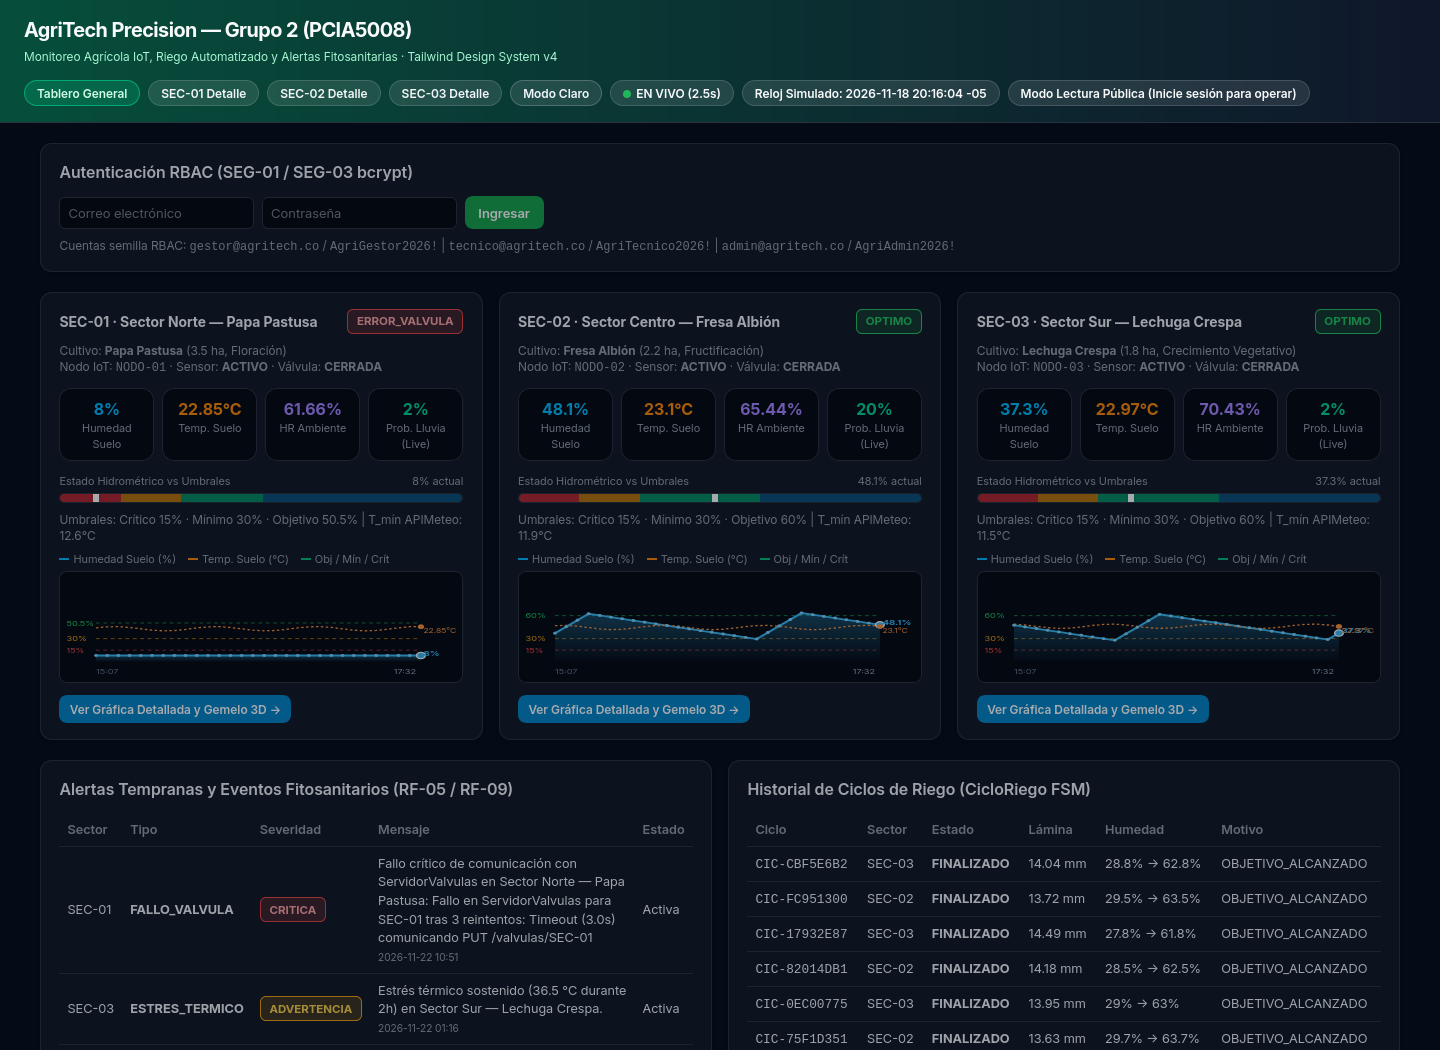
\includegraphics[width=0.96\textwidth]{./figures/vercel_dashboard_live.png}
\caption{Captura real del prototipo \textbf{AgriTech Precision} ejecutándose en producción sobre Vercel (\url{https://agri-tech-six-cyan.vercel.app}), mostrando los tres sectores agrícolas, alertas tempranas, historial de ciclos FSM y gráficas interactivas.}
\label{fig:vercel_live}
\end{figure}

\end{document}
